\documentclass[journal]{IEEEtran}
\usepackage[utf8]{inputenc}
\usepackage{graphicx} % for pdf, bitmapped graphics files
\usepackage{amsmath} % assumes amsmath package installed
\usepackage{amsthm}  % For special theorem style
\usepackage{amsfonts}
\usepackage{dsfont}
\usepackage[USenglish]{babel}  % language support
\usepackage[capitalize]{cleveref}\crefname{equation}{}{}\Crefname{equation}{Equation}{Equations}
\usepackage{siunitx}
\usepackage[nolist,nohyperlinks]{acronym}
\usepackage{xcolor}
\usepackage{csquotes}
\usepackage{tikz}\usetikzlibrary{shapes,arrows,backgrounds}
\usepackage{pgfplots}\pgfplotsset{compat=1.16}
\usepackage{tabularx}
\usepackage{booktabs}\setlength{\heavyrulewidth}{0.1em}\newcommand{\otoprule}{\midrule[\heavyrulewidth]}	



\usepackage{silence}  							%% For filtering warnings
\usepackage[style=ieee,doi=false,isbn=false,url=false,date=year,backend=biber,maxbibnames=15,maxcitenames=2,mincitenames=1,uniquelist=false,uniquename=false,giveninits=true]{biblatex}
% Filter warnings issued by package biblatex starting with "Patching footnotes failed"
\WarningFilter{biblatex}{Patching footnotes failed}
\renewcommand*{\bibfont}{\footnotesize}		%% Use this for papers
\renewcommand*{\bibfont}{\small}
\setlength{\biblabelsep}{\labelsep}
\bibliography{references_rq}



\theoremstyle{remark}\newtheorem{remarkenv}{Remark}        %% remarks
\newenvironment{remark}{\begin{remarkenv}}%
	{\hfill$\lozenge$\end{remarkenv}}            %% end remark with a lozenge



% Notations
\newcommand{\dimension}{d}
\newcommand{\e}[1]{\exp\left\{ #1 \right\}}
\newcommand{\expectation}[1]{\mathds{E}\left[ #1 \right]}
\newcommand{\injury}{\mathrm{injury}}
\newcommand{\numberofencounters}{k}
\newcommand{\parameters}{x}
  \newcommand{\pardim}{d}
\newcommand{\poissonparameter}{\lambda}
\newcommand{\probability}[1]{\mathds{P}\left( #1 \right)}
  \newcommand{\probabilitycond}[2]{\probability{ #1 | #2 }}
\newcommand{\realnumbers}{\mathds{R}}
\newcommand{\scenario}{S}
  \newcommand{\scenarioinstance}[1]{\scenario_{#1}}
\newcommand{\scenariocategory}{\mathcal{C}}
\newcommand{\simulationoutcome}[1]{R\left(#1\right)}


\newcommand{\todo}[1]{\color{red}TO DO: #1 \color{black}}

% Acronyms
\begin{acronym}[AAAAAAAA]
    \acro{acc}[ACC]{Adaptive Cruise Control}\acroindefinite{acc}{an}{an}
    \acro{ads}[ADS]{Automated Driving System}\acroindefinite{ads}{an}{an}
	\acro{av}[AV]{Automated Vehicle}\acroindefinite{av}{an}{an}
	\acro{cmc}[CMC]{Crude Monte Carlo}
	\acro{fcw}[FCW]{Forward Collision Warning}
	\acro{hdm}[HDM]{Human Driver Model}
	\acro{idm}[IDM]{Intelligent Driver Model}
	\acro{idmplus}[IDM+]{Intelligent Driver Model plus}
	\acro{is}[IS]{Importance Sampling}\acroindefinite{is}{an}{an}
	\acro{odd}[ODD]{Operational Design Domain}\acroindefinite{odd}{an}{an}
	\acro{pdf}[pdf]{probability density function}
\end{acronym}


\begin{document}
\date{}

\title{Risk Quantification for Automated Driving Systems in Driving Scenarios}

\author{Erwin~de~Gelder$^{1,2,*}$,
	    Hala~Elrofai$^{1}$,
	    Arash~Khabbaz~Saberi$^{3}$,
	    Jan-Pieter~Paardekooper$^{1,4}$,
	    Olaf~Op~den~Camp$^{1}$,
	    Bart~De~Schutter$^{2}$%
\thanks{$^1$ TNO, Dept.\ of Integrated Vehicle Safety, Helmond, The Netherlands}%
\thanks{$^2$ Delft University of Technology, Delft Center for Systems and Control, Delft, The Netherlands}%
\thanks{$^3$ TomTom, Automated Driving product unit, Eindhoven, The Netherlands}%
\thanks{$^4$ Radboud University, Donders Institute for Brain, Cognition and Behaviour, Nijmegen, The Netherlands}%
\thanks{$^*$ Corresponding author: \textit{erwin.degelder@tno.nl}}}%

\maketitle
\begin{abstract}
	\todo{Write abstract}
\end{abstract}
\acresetall

%%%%%%%%%%%%%%%%%%%%%%%%%%%%%%%%%%%%%%%%%%%%%%%%%%%%%%%%%%%%%%%%%%%%%%%%%%%%%%%%
\section{Introduction}
\label{sec:introduction}

Objective/Research question of the paper: how to quantify safety risk associated with driving automated vehicles 

Suggested structure: 
\begin{itemize}
    \item Context: describe the context of the problem
    \item Background info: short intro to relevant topics: SOTIF, ISO 26262, Scenario based analysis, previous risk quantification efforts, 
    \item Gap: what is missing?  
    \item Contributions: what are we adding in this paper: Adding severity quantification, adding controllability quantification, adding triggering conditions, applying it for multiple relevant scenarios
    \item structure of the paper
\end{itemize}

SOTIF: Absence of unreasonable risk due to hazards resulting from functional inefficiencies of the intended functionality or from reasonably foreseeable misuse by persons.
Hazard identification and evaluation is part of the process to ensure safety according to ISO~21448.
This includes:
\begin{itemize}
    \item Context: 
    Automated driving development requires simulation both at the design phase as well as the assessment phase for covering ``corner'' or ``edge'' cases. 
    Quantifying risk is pivotal for successfully covering the huge ``design space''
    \item Background: 
    Risk is defined by ISO~26262 with three main elements: probability of exposure to the ``\textit{operational situation}'', \textit{severity} of the outcome of scenario, and \textit{controllability} of the situation. 
    \item Determining the probability of exposure of the ``operational situation''.
    \item Determining the \textit{severity} based on models from the literature that depend on parameters such as impact speed. 
    \item Determining the \emph{controllability}, which is defined as ``ability to avoid a specified harm or damage through the timely reactions of the persons involved, possibly with the support from external measures'' \autocite{ISO26262}.
    \item Background continued: SOTIF, as an addition to ISO~26262, is concerned by hazards that are the result of \textit{functional insufficiency} as opposed to \textit{malfunctioning behavior}. Functional insufficiency is either performance limitation or specification issues that could be exposed by a \textit{triggering condition}. Triggering condition is defined in ISO/DIS~21448 as ``specific conditions of a scenario that serve as an initiator for a subsequent system reaction leading to hazardous behaviour.'' 
    
    
    \item Gap: There is not risk quantification method that is able to consider are these factors together. 
    
    \item contribution 1: method for quantifying risk considering exposure, severity, controllability, and triggering condition. 
    \item contribution 2: illustrative case studies on several scenarios and triggering conditions: 
    TODO: make a list of scenarios. 
    
    

\end{itemize}

\section{Method}
\label{sec:method}



\section{Case study}
\label{sec:case study}



\subsection{Automated driving system under test}
\label{sec:ads under test}



\subsection{Scenario categories}
\label{sec:scenario categories}



\subsection{Triggering conditions}
\label{sec:triggering conditions}

\section{Results}
\label{sec:results}

\todo{Write introduction for this section.}



\subsection{Risk of false positives}
\label{sec:results false negatives}

\todo{Make sure colors are consistent through the different images}

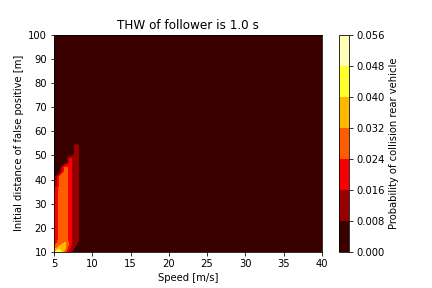
\includegraphics[width=.9\linewidth]{figures/fp_prob_10_100_5_40_10.png}

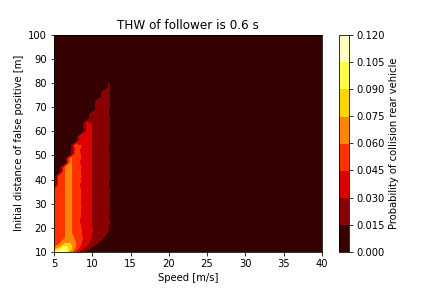
\includegraphics[width=.9\linewidth]{figures/fp_prob_10_100_5_40_06.png}

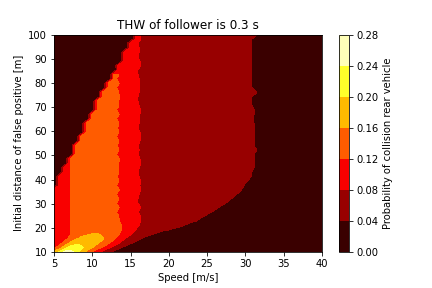
\includegraphics[width=.9\linewidth]{figures/fp_prob_10_100_5_40_03.png}

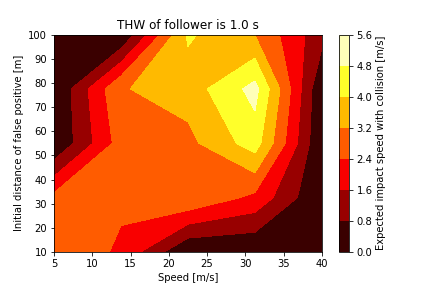
\includegraphics[width=.9\linewidth]{figures/fp_vimpact_10_100_5_40_10.png}

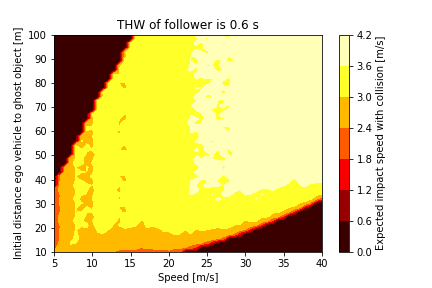
\includegraphics[width=.9\linewidth]{figures/fp_vimpact_10_100_5_40_06.png}

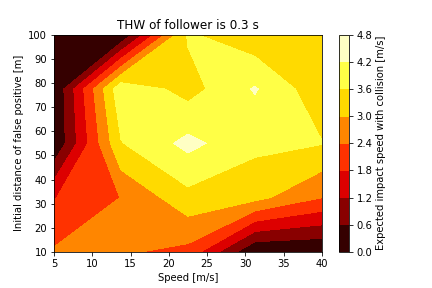
\includegraphics[width=.9\linewidth]{figures/fp_vimpact_10_100_5_40_03.png}



\subsection{Risk of false negatives}
\label{sec:results false positives}

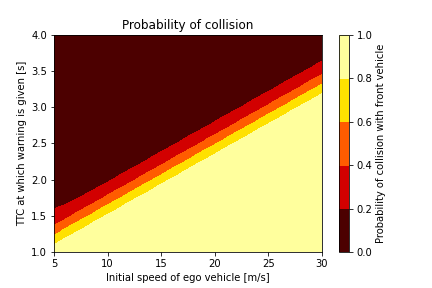
\includegraphics[width=.9\linewidth]{figures/fn_prob_v5_30_ttc1_4.png}

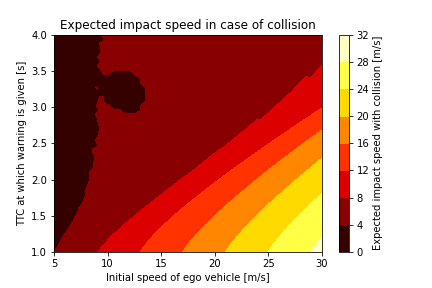
\includegraphics[width=.9\linewidth]{figures/fn_vimpact_v5_30_ttc1_4.png}




\subsection{Risk of low-$\mu$ road surface}
\label{sec:results low mu}



\subsection{Risk of graded road}
\label{sec:results slope}

\acresetall
\section{Conclusions}
\label{sec:conclusions}





\printbibliography

\end{document}
